\documentclass[aps,letterpaper,11pt]{revtex4}

\usepackage{graphicx}
\usepackage{float}
\usepackage{verbatim}
\usepackage{amsmath}
\usepackage{amssymb}

\newcommand{\labno}{5}
\newcommand{\labtitle}{Analyzing Force in Systems Using Newton's Laws of Motion}
\newcommand{\authorname}{Kevin Truong}
\newcommand{\professor}{Dr. Melanie Lutz}
\newcommand{\classno}{Physics 006}
\newcommand{\labpartners}{Sean Casey, Kevin Castillo, and Dulce Payan}
\newcommand{\submitdate}{March 7,2017}

\begin{document}

\begin{titlepage}
\begin{center}
\hspace{-136mm}\boxed{{\Large \textsc{Lab No. \labno}}}\\\vspace{30mm}
{\Large \textsc{\labtitle} \\ \vspace{4pt}}
\rule[13pt]{\textwidth}{1pt}\\ \vspace{150pt}
{\large By: \authorname \\ \vspace{10pt}}
Lab Partners: \labpartners \\
Instructor: \professor \vspace{10pt} \\
Solano Community College\\ \classno \\ \vspace{10pt}
\submitdate
\end{center}
\end{titlepage}

\section{Abstract}

The experiment examined Newton's third law by analyzing three different collisions. When two carts (with the same mass) move towards each other with the same speed, one cart moves towards another cart that is at rest, and two carts (with different masses) move towards each other with the same speed. The data collected through all of the collisions prove that Newton's third law holds true, where the maximum force values were the same for both carts in each collision just in different directions. During the first collision Force 1 had a maximum value of -11.46N and Force 2 had a maximum value of 11.02N, indicating that the force during the impact was almost identical but in opposite directions. During the second collision Force 1 (the moving cart) had a maximum force value of -4.16N while Force 2 (the cart at rest) had a maximum force value of 4.19N, which indicated that Newton's third law holds true. During the third collision Force 1 (the cart with higher mass) had a maximum force value of -10.68N while Force 2 had a maximum force value of 10.80N, which indicated that Newton's third law holds true. 

Newton's second law was also analyzed, using the Force Vs. Acceleration graph the mass was found by analyzing the slope of the trendline of the graph, which was .740kg. It was determined that mass was the slope of the Force Vs. Acceleration graph because of the equation $m = \frac{F}{a}$ which was derived from Newton's second law. The actual mass was found using a scale, which was .688kg. The percent error from the calculated mass and the actual mass was 7.56\%.

\section{Introduction}

To understand forces and its applications, it's important to understand Newton's three laws of motion. Newton's first law states that every object persists in a state of rest or uniform motion unless a force is applied to the object. The second law states that the summation of forces on a body is equal to the mass times the acceleration of the body, which is well known as the famous equation: $F = ma$ where F is force, m is mass, and a is acceleration. Newton's Third law states that for every action, there is an equal and opposite reaction. 

Analyzing accuracy in data is important in understanding the possible flaws that occur during experiments. Calculating percent error in this experiment was accomplished by using the equation: $\%\hspace{1mm}error = \frac{m_{exp}-m}{m}*100\%$.


\section{Experimental Details}

Equipment for this experiment includes a force sensors, impact reader, carts, "frictionless" ramp, motion sensor, and computer. The force sensors measure the force of the collision of the two carts by measuring the change in voltage due to the bending of the metal. The impact reader was used to measure the force of the collisions. The carts held the force sensors and was the contraption that transported the force sensor and created the collision. The "frictionless" ramp was where the carts were placed to omit friction from the data. The motion sensor was used in part B of the experiment to collect the acceleration of the cart when a force is applied to the cart.The computer was used to collect and process the data of the change of voltage picked up by the force sensors using the Logger Pro Program. 

This experiment examined how Newton's laws worked by exploring the basic properties of forces using the collision of carts in different scenarios to show that Newton's third law holds and the relationship between acceleration and force for Newton's second law. 

In part A of the experiment, two force sensors and impact readers were used to calculate the force of the collision between two carts, showing that Newton's third law holds true. After calibrating and connecting the force sensors to the Logger Pro Program on the computer, the force sensors were attached on top of the carts. Three different collisions were examined: while the two carts(with the same mass) were moving towards each other with the same speed, one cart moving towards a cart at rest, and two carts(with different masses) moving towards each other with the same speed. Diagram One shows the setup for part A.

\begin{center}
\underline{Diagram 1}\\
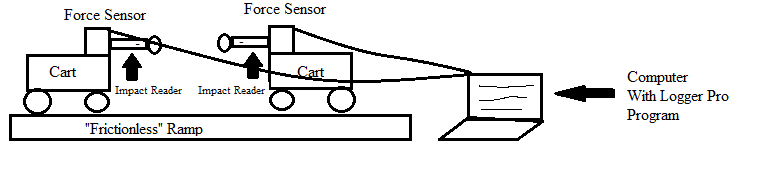
\includegraphics[width=6in]{SetupPartA.png}\\
\textit{Diagram 1: Setup for Part A, analyzing Newton's Third Law}\\
\end{center}

In part B of the experiment, a motion sensor was used to analyze the acceleration of the cart due to a force applied. This part of the experiment will use Newton's second law to analyze the mass. The cart with the force sensor was dragged back and forth on the frictionless ramp. Diagram two shows the setup for part B.

\begin{center}
\underline{Diagram 2}\\
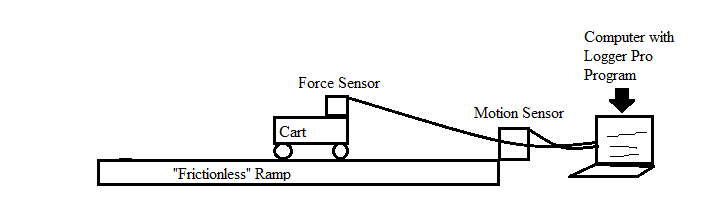
\includegraphics[width=6in]{SetupPartB.png}\\
\textit{Diagram 2: Setup for Part B, analyzing Newton's Second Law}
\end{center}

It's important to note that the force sensors need to be calibrated before use, a 1kg hanging mass was used to model 9.8 N of force.


\section{Results and Analysis}

\subsection{Newton's Third Law}

Newton's Third Law applies to all forces that act on each other. To demonstrate this, three different collisions were conducted in the experiment. First collision involved both carts moving towards each other at the same speed. Figure one was the result of the collision for both carts colliding at the same speed (collision one).

\newpage

\begin{center}
\underline{Figure 1}\\
\vspace{-10mm}
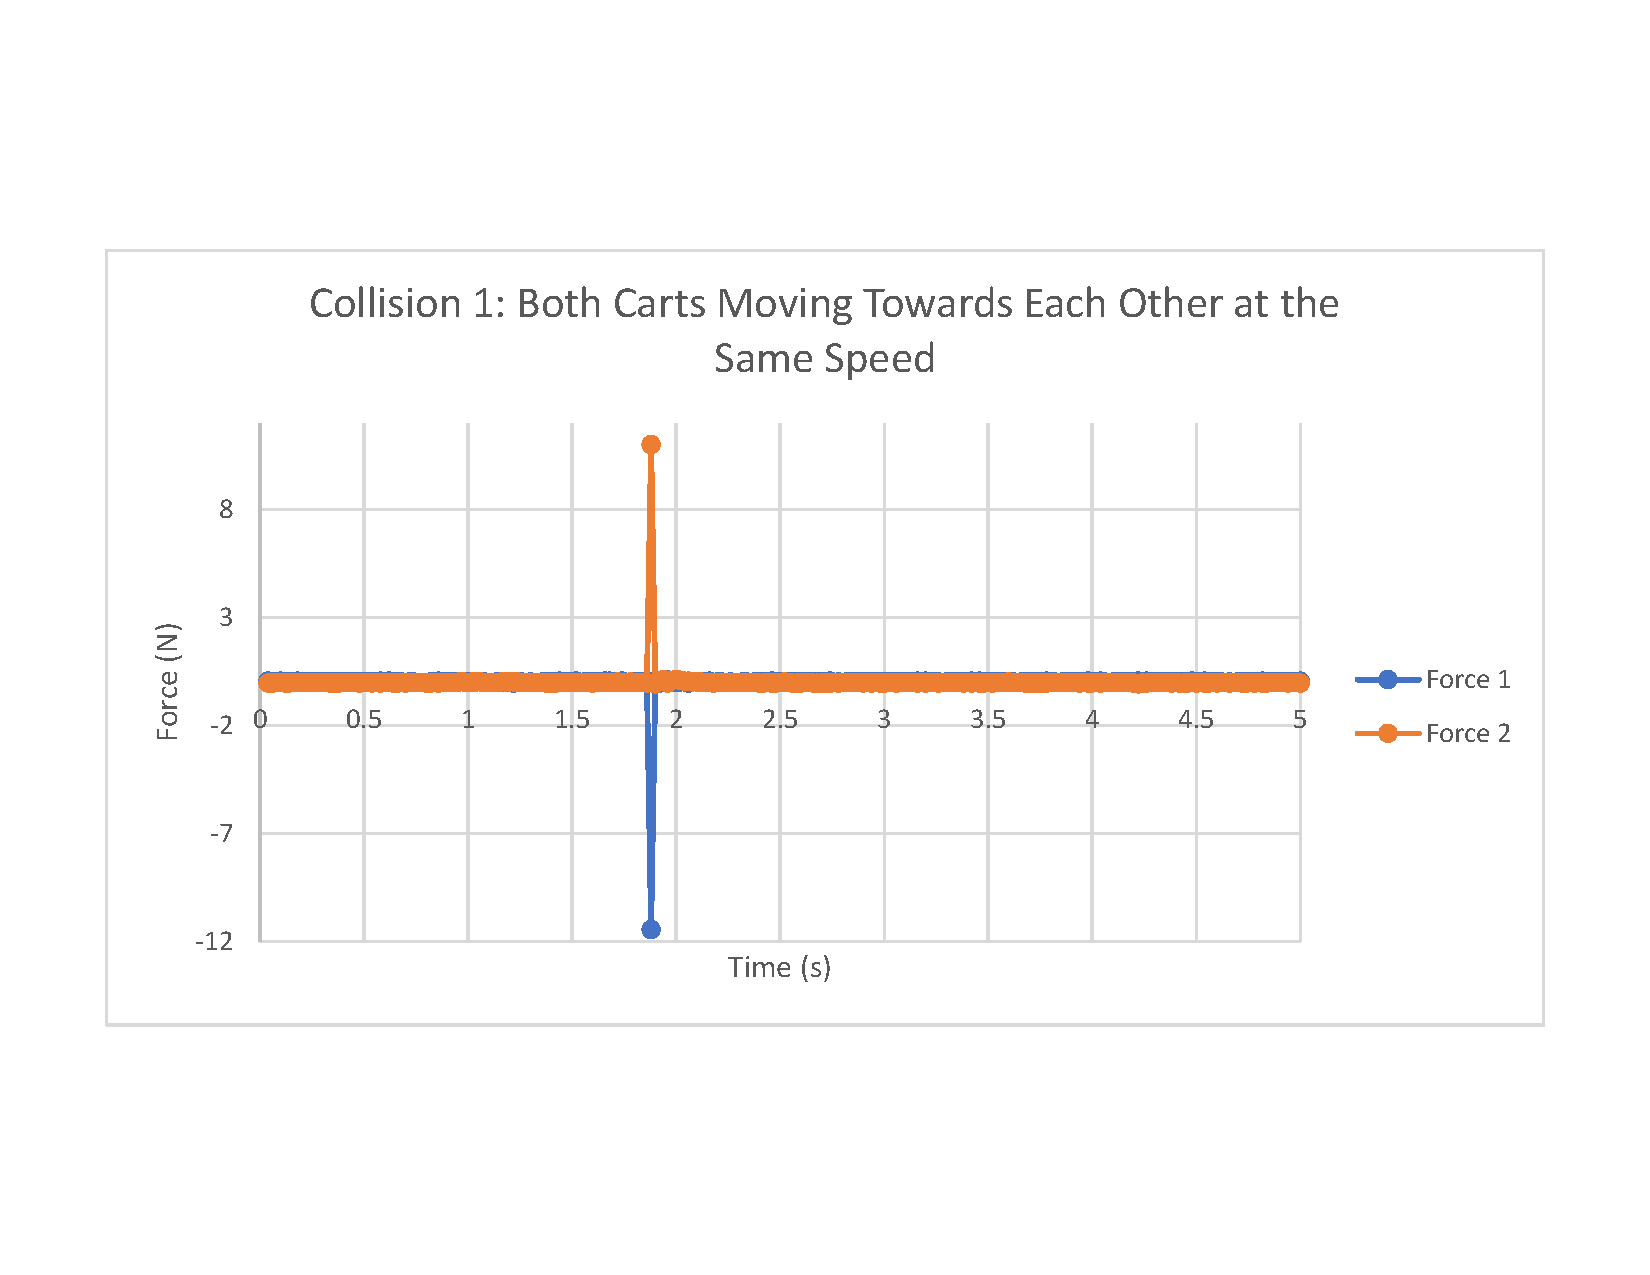
\includegraphics[width=6in]{FirstCollisionGraph.pdf}\\
\vspace{-10mm}
\textit{Figure 1: The graph of both carts, with the same mass, colliding at the same speed. The graph shows that Force 1 (the pulling force) exerted an equal but opposite force on Force 2 (the pushin force).}
\end{center}

Newton's Third Law states that if body A exerts a force, F, on body B, then body B will exert that exact same force, F, in the opposite direction at exactly the same time. The collision modeled in Figure one shows that "Force 1" exerted an equal and opposite force on "Force 2," at exactly the same time. It's important to note that Force 1 was calibrated as a negative force value and Force 2 was calibrated as a positive force value, so the spike (which occured at exactly the same time) was easily visible. The following data table shows the time interval, maximum force, and mean force of collision one. 

\begin{center}
\underline{Data Table: Collision One}\\
\begin{tabular}{ |c|c|c| }
\hline
 & Cart 1 (Force 1) & Cart 2 (Force 2)\\
\hline
Time Interval (s) & 0.04 (1.86-1.90) & 0.04 (1.86-1.90)\\
\hline
Maximum Force (N) & -11.46 & 11.02\\
\hline
Mean Force (N) & -1.112 & 1.111\\
\hline
\end{tabular}
\end{center}

The data table above shows that Newton's third law holds true in the first collision. Since the magnitude of the maximum force and the mean force is nearly identical, the data proves that Newton's third law holds true. Cart one's values are negative because of the way the cart was calibrated in the beginning of the lab. The maximum value of Force 1 and Force 2 occur at 1.88s. The time interval in which the maximum force occurs is 1.86s to 1.90s. From this result, collision one demonstrated that Newton's third law holds true because both maximum forces occur at exactly the same time, with almost identical forces, and with nearly identical mean forces. 

The second collision involved Force 1 (cart one) moving at some speed and colliding with Force 2(cart two) which was at rest; Figure two is the graphical result of this collision.

\begin{center}
\underline{Figure 2}\\
\vspace{-10mm}
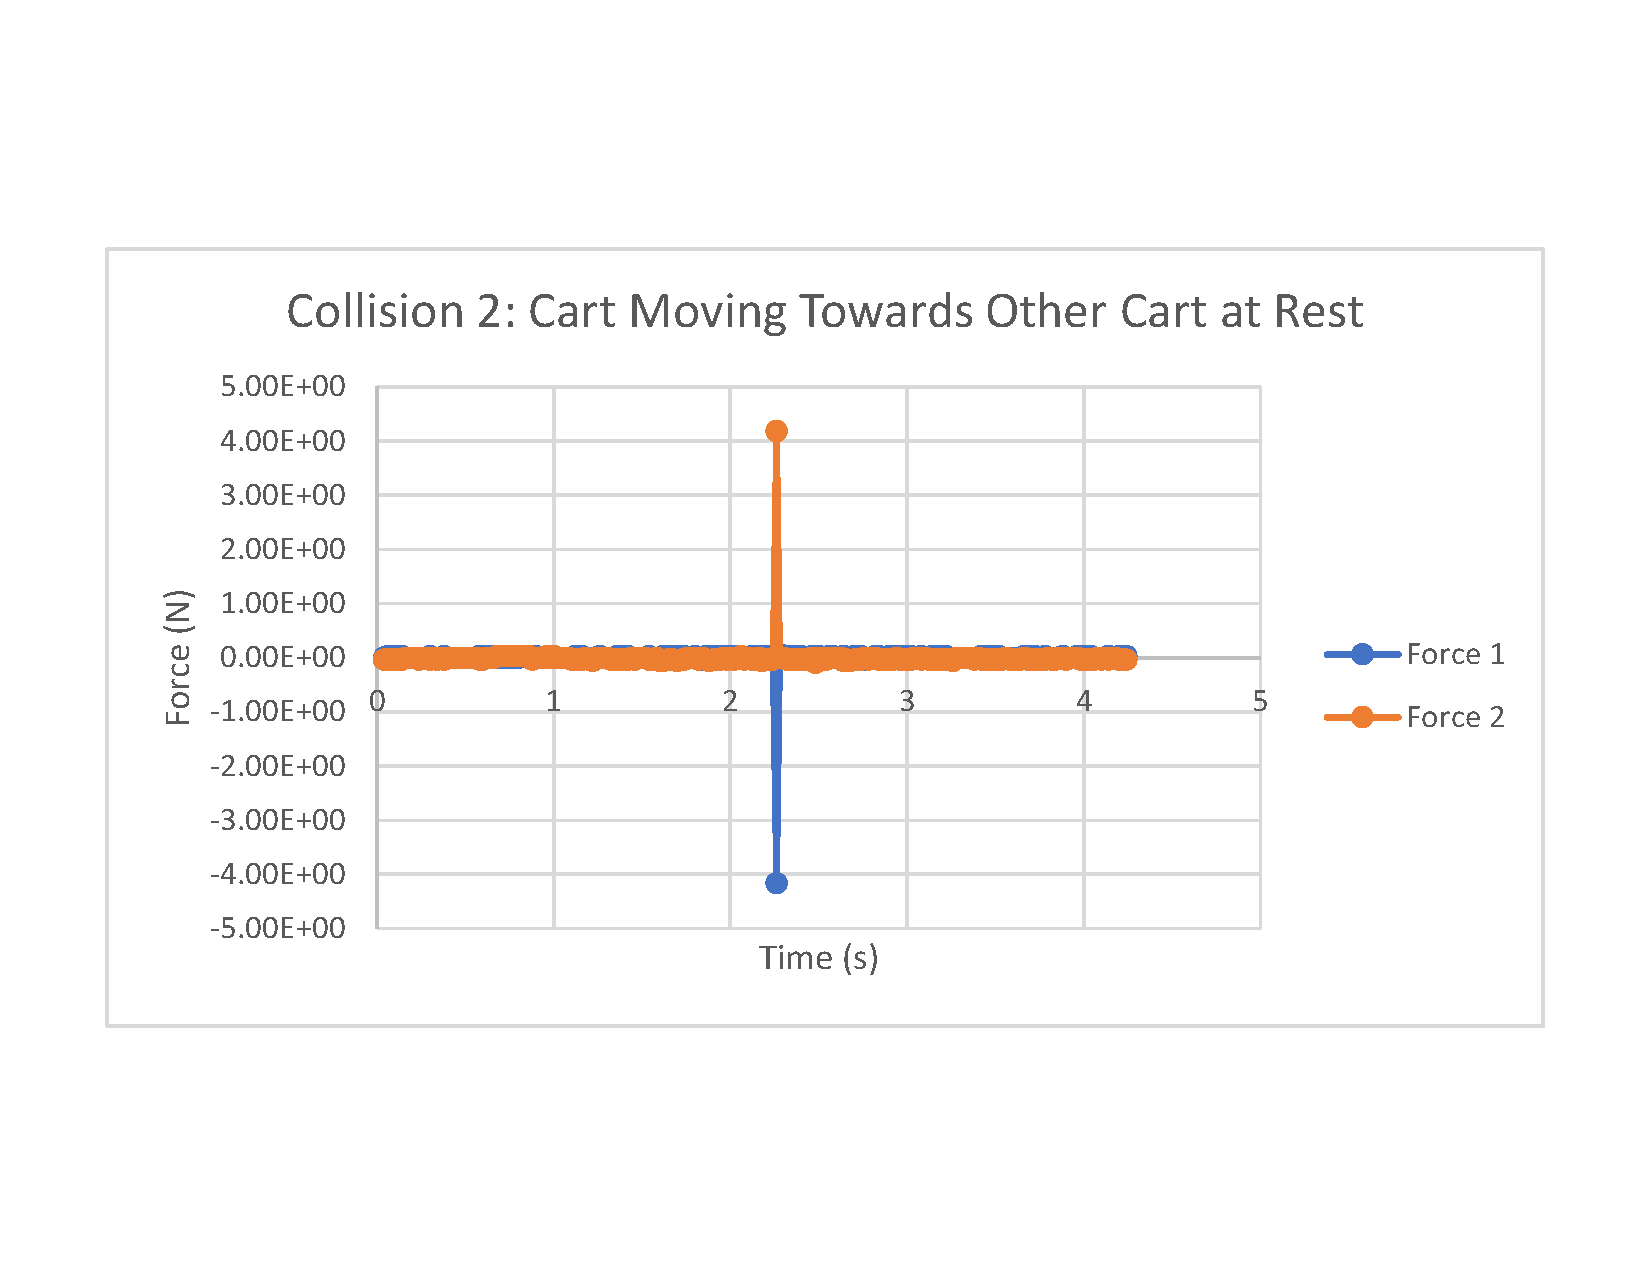
\includegraphics[width=6in]{SeconCollisionGraph.pdf}\\
\textit{Figure 2: Graph of cart one (Force one) colliding with cart two (cart two) which was at rest. }
\end{center}

Figure two shows that Force 1 (the pulling force) exerted an equal and opposite force on Force 2 (the pushing force). Similar to collision one, collision two demonstrated a similar result with Force 1 exerting an equal and opposite force on Force 2. At the moment of collision, Force 1 and Force 2 spike to extreme negative and positive values, respectively. The following table shows that the magnitude of the extremas that the forces reached are almost identical. 

\newpage

\begin{center}
\underline{Data Table: Collision Two}\\
\begin{tabular}{|c|c|c|}
\hline
 & Cart 1 (Force 1) & Cart 2 (Force 2)\\
 \hline
 Time Interval (s) & 0.04 (2.24-2.28) & 0.04 (2.24-2.28)\\
 \hline
 Maximum Force (N) & -4.16 & 4.19\\
 \hline
 Mean Force (N) & -0.359 & 0.356\\
 \hline
\end{tabular}
\end{center}

According to the data collected, the magnitude of the maximum force and mean force of Force 1 and Force 2 are almost identical. The maximum force of both carts happen at exactly the same time interval: from 2.24s to 2.28s. The data shows that the carts had equal and opposite forces at exactly the same time. Even though Force 2 was at rest before the collision, Newton's third law still holds true. 

The third collision is exactly the same as the first collision, but this time cart one (Force 1) has more mass than cart two (Force 2). Figure three was the graphical result of the third collision with one cart having more mass than the other.

\begin{center}
\underline{Figure 3}\\
\vspace{-10mm}
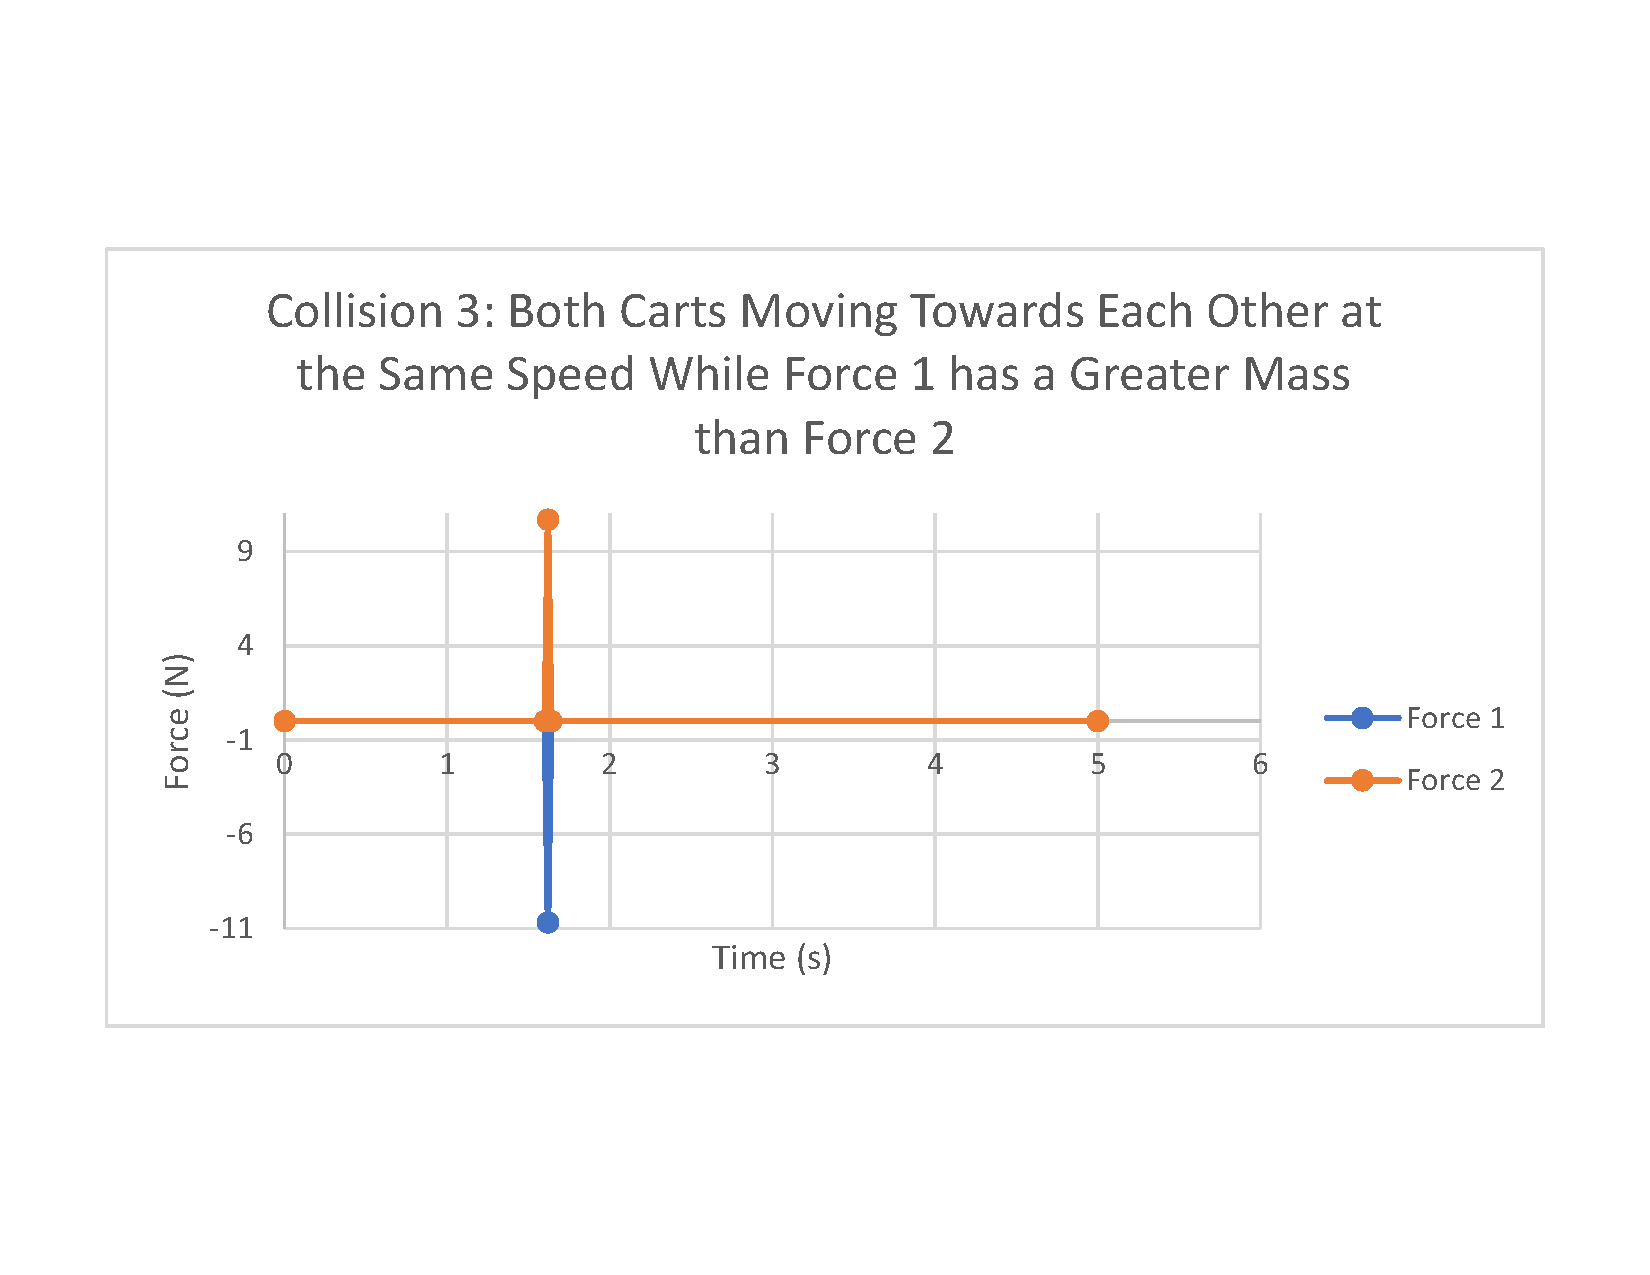
\includegraphics[width=6in]{Collision3Graph.pdf}\\
\textit{Figure 3: Graph of Force 1 (with more mass) colliding with Force 2. Again the graph shows that Force 1 (the pulling force) exerted an equal and opposite force on Force 2 (the pushing force) at exactly the same time}
\end{center}

The third collision demonstrated similar results as collision one and two, where Force 1 is exerting an equal and opposite force with Force 2. At exactly the same time, the forces for both Force 1 and Force 2 spiked to extremas that have nearly identical magnitudes. The following data table shows the time interval of the collision, the maximum force achieved, and the mean force. 

\begin{center}
\underline{Data Table: Collision Three}\\
\begin{tabular}{|c|c|c|}
\hline
 & Cart 1 (Force 1) & Cart 2 (Force 2)\\
 \hline
 Time Interval (s) & 0.04 (1.6-1.64) & 0.04 (1.6-1.64)\\
 \hline
 Maximum Force (N) & -10.68 & 10.90\\
 \hline
 Mean Force (N) & -1.78 & 1.81\\
 \hline
\end{tabular}
\end{center}

The table above is the important data from the third collision, and it shows that Cart 1 and Cart 2 have almost identical magnitudes of maximum force and mean force. It also shows that the extremas occur at the exact same time interval: 1.60s to 1.64s. Just like in the first and second collision, the data shows that the collision resulted in forces that were equal and opposite; which shows that Newton's third law holds true even when one cart has more mass than the other. However, it is important to note that the maximum force that occured during the third collision was less than the maximum force that occured in the first collision. The maximum force should be more in the third collision, compared to the first collision, if the acceleration in both collisions were the same due to the cart having more mass in collision three. Newton's second law, F=ma, explains that the maximum force should be higher in the collision that had a higher mass if the acceleration was the same. The disparity in this result must have been due to the person-pushing-the-carts not pushing them together at the same acceleration, causing the first collision to have more acceleration which resulted in the higher maximum force. 

Newton's third law held true in all three collisions. If one cart exerts a force on a second cart, the second cart will exert the exact force back onto the first cart at exactly the same time. Newton's third law is always true when two objects come into contact with each other.

\subsection{Newton's Second Law}   

Newton's second law states that $F = ma$, indicating that there is a directly proportional relationship between force and acceleration. This relationship can be seen in the mess up that occured between collision one and collisions three. The maximum force that occured in the third collision should be more than the maximum force that occured in the first collision when both systems have the same acceleration because the mass of the cart in the third collision was more than the mass in the first collision; however, the maximum force in the first collision was more than the maximum force in the third collision. The reason for this result must be due to the acceleration in the first collision being greater than the acceleration in the third collision.  

In this part of the lab we used a motion sensor to collect the acceleration of the cart while a force is being applied. One cart was pulled and pushed back and forth in front of a motion sensor to obtain multiple force and acceleration readings. Since force and acceleration are directly proportional the graph of force vs. acceleration should be a linear graph, where the change in one directly changed the other in the same manner. For example, if acceleration is decreased the force should also decrease or if force is increased the acceleration should increase as well. Figure four shows the graphical representation of the $F = ma$ and the directly proportional relationship between force and acceleration. Figure four also shows all of the data that was collected from moving the cart back and forth and collecting the force and accelerations of the cart. 

\begin{center}
\underline{Figure 4}\\
\vspace{-50mm}
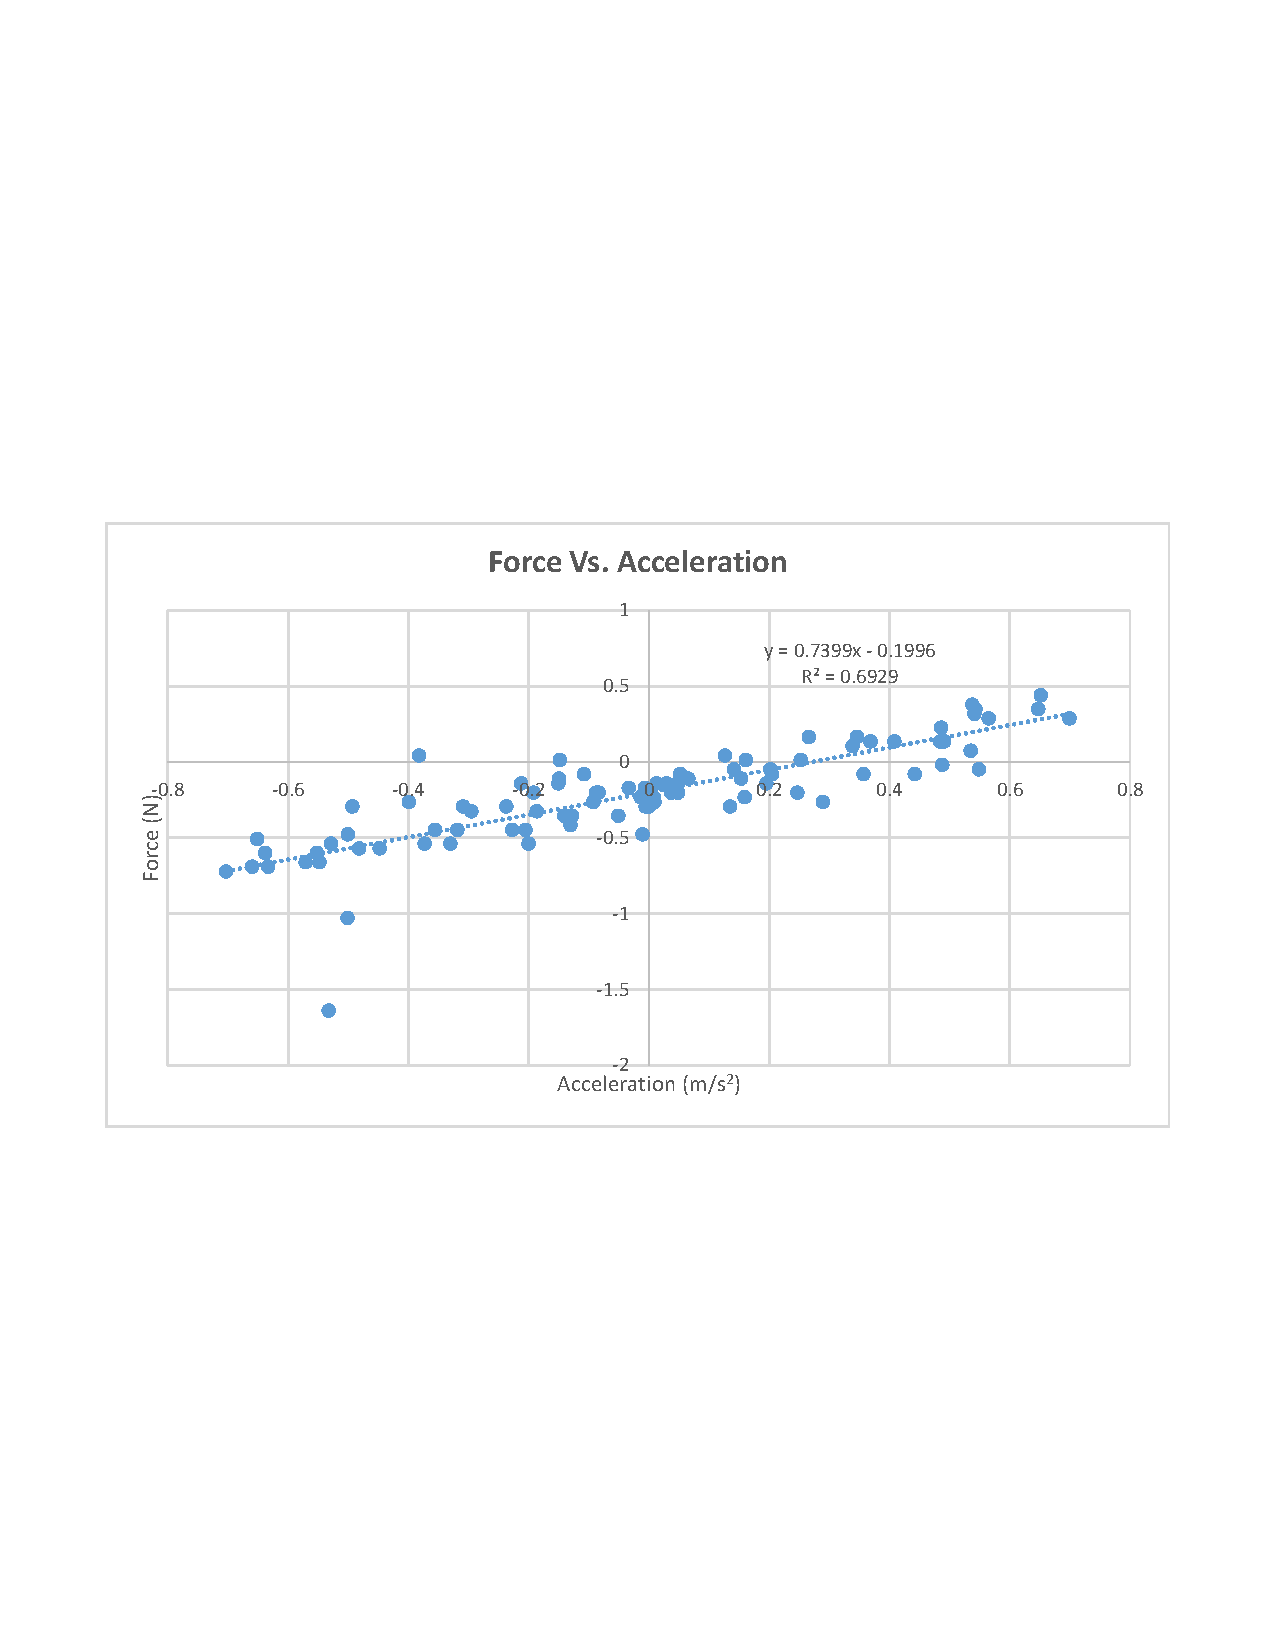
\includegraphics[width=5in]{FinalDataAccelerationForceGraph.pdf}\\
\vspace{-50mm}
\textit{Figure 4: The Force Vs. Acceleration graph of the cart in part B}
\end{center}

The trendline in the Force Vs. Acceleration graph represents the general behavior of force and acceleration, showing that as one increases the other also increases in a linear fashion. The slope of the trendline is the mass of the object, this can be easily seen by solving for mass in the $F = ma$ equation. When solving for mass, the equation becomes: $m=\frac{F}{a}$, which explicitly shows that mass is just the slope of the force vs. acceleration graph. Through the equation of the trendline, the slope of the equation was 0.7399; therefore the calculated mass of the cart was 0.7399kg. The cart was then measured with a gram scale to obtain the actual weight of the cart, which was 0.688kg. To show the accuracy of the calculated mass with the actual mass of the cart, the percent error was calculated. Using the following formula the calculation was possible:

$$ \% \hspace{1mm}error = \frac{m_{exp}-m}{m}*100\%$$ 

The calculated percent error for the mass was 7.56\%. This means that the percent error between the calculated mass and the actual mass of the cart from the experiment was 7.56\%, which was within the range for accuracy of the mass.

\section{Discussion} 

Newton's third law applies to any type of collision, whether the two objects are moving at the same speed, an object collides with another object at rest, an object with a higher mass colliding with an object with a smaller mass, or any other collision. Through the first, second, and third collision Newton's third law holds true. The maximum forces were different throughout the collision could have been attributed to the person-pushing-the-carts not pushing the carts with the same acceleration causing one collision to have greater force than the others. 

The directly proportional relationship between force and acceleration of an object can be represented in Newton's second law: $F = ma$. If the acceleration of an object increases, the force of the object also increases. The mass of an object was derived using the same equation, $m = \frac{F}{a}$, this shows that mass is the slope of the Force Vs. Acceleration graph. After calculating the mass of the cart looking at the trendline of the Force Vs. Acceleration graph, it was calculated that the percent error was 7.56\%. This percent error could be attributed to equipment inaccuracies.   

\section{References}

\hspace{-6.5mm}
Force and Acceleration I Physics 06 Lab, Dr. Melanie Lutz\\



\end{document}
